\documentclass[a4paper]{llncs}
\usepackage{amsmath}

\usepackage{tikz}
\usetikzlibrary{positioning}
\usetikzlibrary{calc}
\usetikzlibrary{arrows,shapes,backgrounds}

\newcommand{\vphi}{\vec{\varphi}}
\newcommand{\vi}{{\vec{i}}}
\newcommand{\vj}{{\vec{j}}}
\newcommand{\vmu}{\vec{\mu}}

\title{ GPU-accelerated and CPU SIMD Optimized \\ Monte Carlo Simulation of $\phi^4$ Model}
\author{Piotr Bialas\inst{1} \and Jakub Kowal\inst{1} \and Adam Strzelecki\inst{1}}
\institute{Faculty of Physics, Astronomy and Applied Computer Science\\
Jagiellonian University\\
ul. Reymonta 4, 30-059 Krakow, Poland }
\begin{document}


\maketitle


\section{The model}
This contribution is concerned with an efficient implementation of the
Monte-Carlo simulations of the $\varphi^4$ model. The problem is
defined as follows: having a vector field $\vphi$ defined on a regular
rectangular two or three dimensional grid we want to generate the field configurartions with probability proportional to
\begin{equation}
e^{-H(\vphi)}
\end{equation}
where 
\begin{equation}\label{eq:ham}\begin{split} 
H(\varphi)&=\sum_{\vi}\Biggl(
\frac{1}{2}\sum_{\mu=1}^d(\vphi_{\vi+\hat{\mu}}-\vphi_{\vi})^2
+\frac{\mu^2}{2}|\vphi_{\vi}|^2+
\frac{g}{24}(|\vphi_{\vi}|^2)^2\\
&\phantom{=\sum_{\vi}\bigl(}+
\frac{1}{2\Lambda}\Bigl(\sum_{\mu=1}^d(\vphi_{\vi+\hat{\mu}}-2\vphi_{\vi}+\vphi_{\vi-\vmu})\Bigr)^2\Biggr).
\end{split}
\end{equation}
In the above expression $\vi$ denotes the grid point,
$\vphi_\vi$ denotes the $N$ component vector at the grid point $\vi$
 and $\vmu$ denotes the unit displacement on the grid in direction $\mu$. 

The actual  generation is done by the mean of the Metropolis  algorithm as follows: for a given lattice point $\vj$ we produce a new field 
\begin{equation}
\widetilde{\vphi}_\vj=\vphi_\vj+\vec{\epsilon}
\end{equation}
where $\epsilon$ is some random vector. The we calculate the difference 
$\Delta H = H(\widetilde{\vphi})-H(\vphi)$.
We then replace $\vphi_\vj$ with $\widetilde{\vphi}_\vj$ with the probability
\begin{equation}
P=\max\left\{1,\exp(-\Delta H)\right\}.
\end{equation}
The crucial feature of this algorithm is that the $\Delta H$ depends
only on the imediate neighbourhood of the point $\vj$. In our case
because of the lats term in \eqref{eq:ham} this neigborhood is
extended compared to usual nearest neigbours (see figure~\ref{fig:nn}). 
\begin{figure}
\begin{center} 
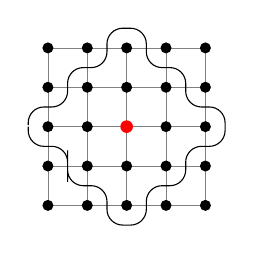
\begin{tikzpicture}[scale=0.5]
%\draw[->,rounded corners=0.2cm,shorten >=2pt] (0,2)-- (1,2);
%\draw (0,0) grid (4,4);
\draw[help lines] (0.0,0.0) grid (4.0,4.0);    

%punkty
\foreach \c in {(0,0),(0,1),(1,0),(4,4),(4,3),(3,4),(0,4),(0,3),(3,0),(4,0),(1,4),(4,1),(2,1),(1,2),(3,2),(2,3),(1,1),(1,3),(3,1),(3,3),(0,2),(4,2),(2,0),(2,4)}
    \fill \c + (0.0,0.0) circle (0.14);

%punkt dla ktorego dokonujemy aktualizacji    
\fill[red] (2,2) circle(0.16);    

%zasieg sasiedztwa    
\draw[rounded corners=0.2cm,shorten >=2pt]
	(-0.5,2.0)-- ++(-0,-0.5)-- ++(1,0)-- ++(-0,-0.5)-- ++(-0,-0.5)-- ++(1,0)-- ++(-0,-1.0)-- ++(1,0)
	-- ++(-0,1.0)-- ++(1,0)-- ++(-0,1.0)-- ++(1,0)-- ++(0,1)-- ++(-1,0)-- ++(0,1)-- ++(-1,0)-- ++(0,1)
	-- ++(-1,0)-- ++(0,-1)-- ++(-1,0)-- ++(0,-1)--  ++(-1,0)-- ++(0,-0.6);   
 
    
%end
\end{tikzpicture}
\end{center}
\caption{\label{fig:nn}The neighbourhood used to update the center point.}
\end{figure}

Two points of the lattice can be updated in parallel provided they do
not belong to other point neigborhood. The neigborhoods themselves can
overlap. We had to devise a way of partitioning the lattice into disjoint sublattices such that points on each partition can be updated simultaneously. In two dimensions this required eight partitions (see figure~\ref{fig:nn})  and 16 in case of three dimensions. 


\end{document}
